\documentclass{article}
\usepackage{graphicx}
\usepackage{amsmath}
\usepackage{array}

\begin{document}

\section*{30. November 2023}



\subsubsection*{Brain, Computer similarity, differences}

\begin{center}
\begin{tabular}{ |m{6em}|m{10cm}| }
\hline
Similar & Different \\
\hline
Process information & Massive parallelism \\
Logical operations & Separation of memory and processing \\
Memory & Constantly adapting \\
Use electrical(digital) signaling & Chemical signaling \\
Can learn from inputs & Unreliable units \\
Consume energy & Analog computation \\
 & Robust to damage \\
 & Very energy efficient \\
\hline
\end{tabular}
\end{center}

\subsubsection*{Lecture 2, Brain}



\section*{Lecture 6, Synapsis}

\subsection*{Soup vs Spark}

\begin{itemize}
    \item is synaptic transmission mediated chemically or by direct electrical transfer of charge
    \item NMJ accepted that it was chemical $\rightarrow$ certain aspects too fast to be mediated chemically
\end{itemize}

\subsection*{Frog experiment}

\begin{itemize}
    \item to support neurotransmitter hypothesis
    \item first frogs heartbeat slowed, second frog inhibitory effect of vagus transferred
    \item building connection of synapsis not rebuilding brain
\end{itemize}

\section*{Lecture 7}

\begin{figure}[h]
\centering
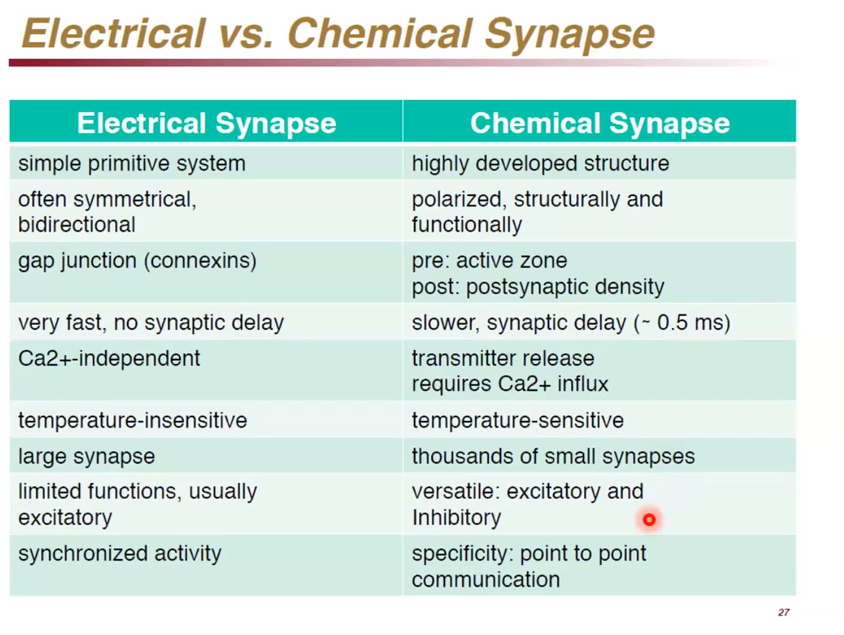
\includegraphics[width=0.5\textwidth]{assets/synapse.png}
\caption{Synapse}
\end{figure}

\section*{Brain Structure}

\noindent \textbf{Telencephalon Regions}

The cerebral cortex (neocortex) is anatomically divided into 4 lobes

\begin{figure}[h]
\centering
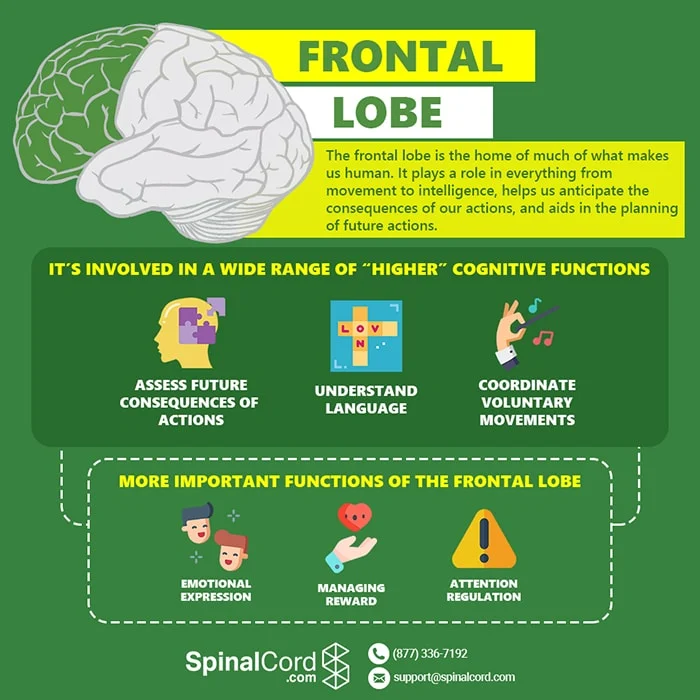
\includegraphics[width=0.5\textwidth]{assets/frontalLobe.png}
\caption{Frontal lobe}
\end{figure}

\begin{figure}[h]
\centering
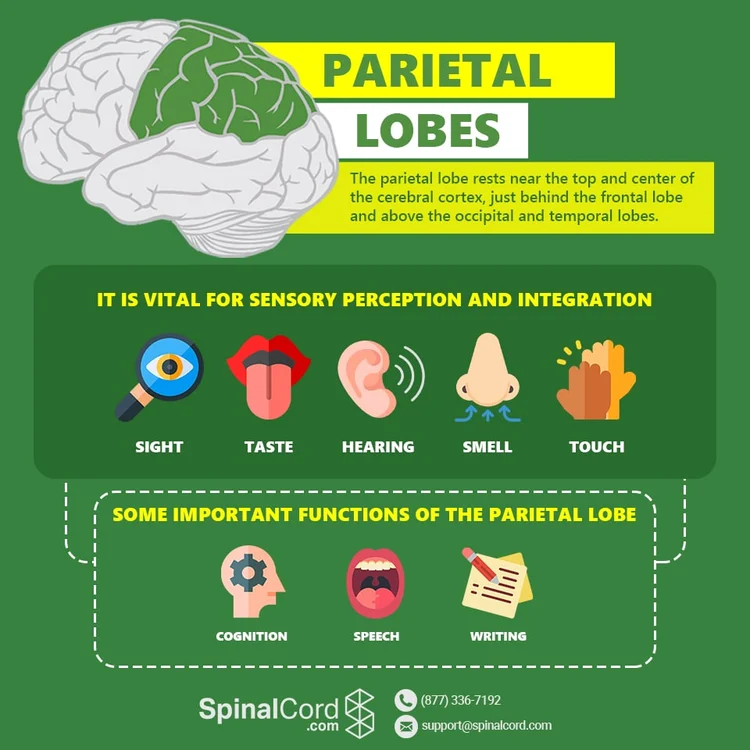
\includegraphics[width=0.5\textwidth]{assets/parietalLobe.png}
\caption{Parietal lobe}
\end{figure}

\noindent separated from the frontal lobe by the \textbf{central sulcus}. Primary lobe for somatosensory processing (afferent inputs from receptors in the skin). Additionally, subserves other sensori-motor functions.

\begin{figure}[h]
\centering
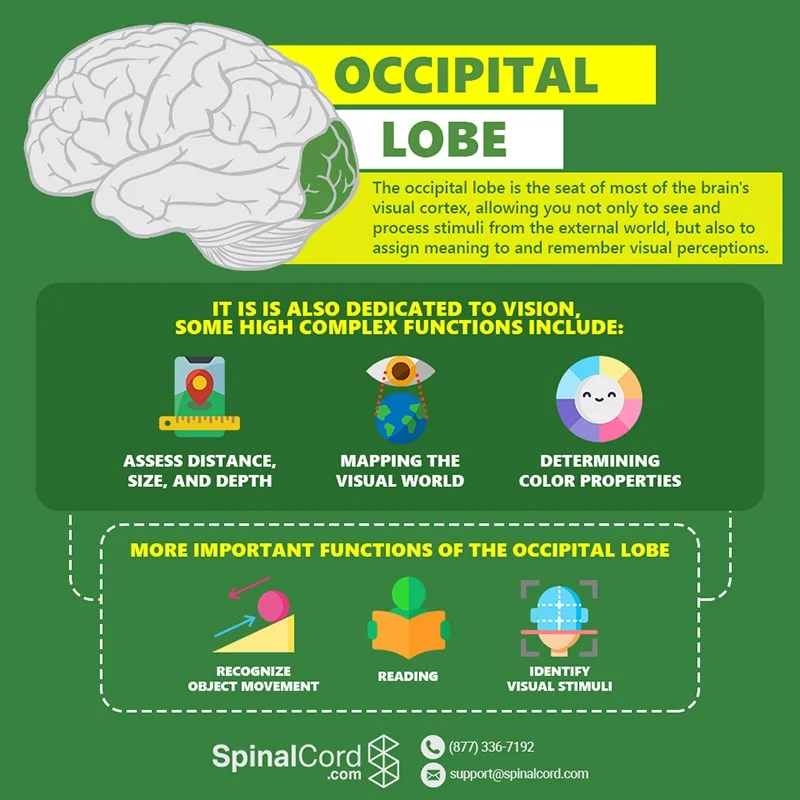
\includegraphics[width=0.5\textwidth]{assets/occipitalLobe.png}
\caption{Occipital lobe}
\end{figure}

\begin{figure}[h]
\centering
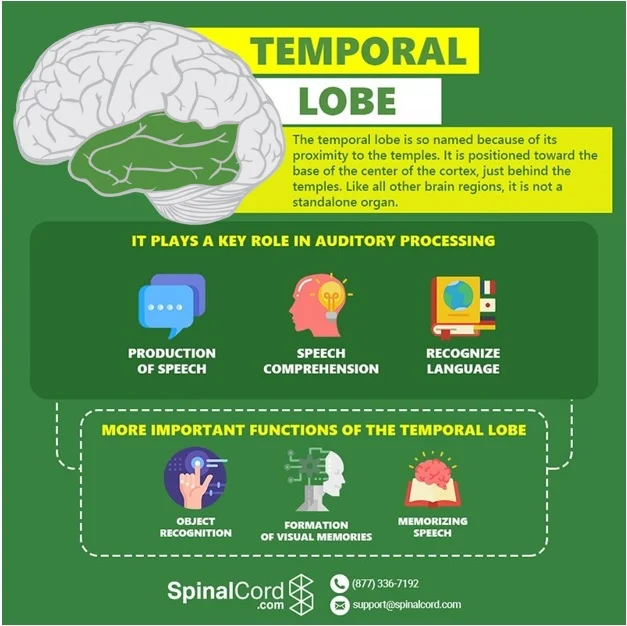
\includegraphics[width=0.5\textwidth]{assets/temporalLobe.png}
\caption{Temporal lobe}
\end{figure}

\noindent separated from the frontal and parietal lobe by the \textbf{lateral fissure (Sylvian fissure)}. Involved in auditory processing and language comprehension \textbf{(Wernickes area)}. Additionally, responsible for visual object recognition. The medial portion of the temporal lobe includes a \textbf{portion of the hippocampal formation which is involved in formation of new memories}

\begin{figure}[h]
\centering
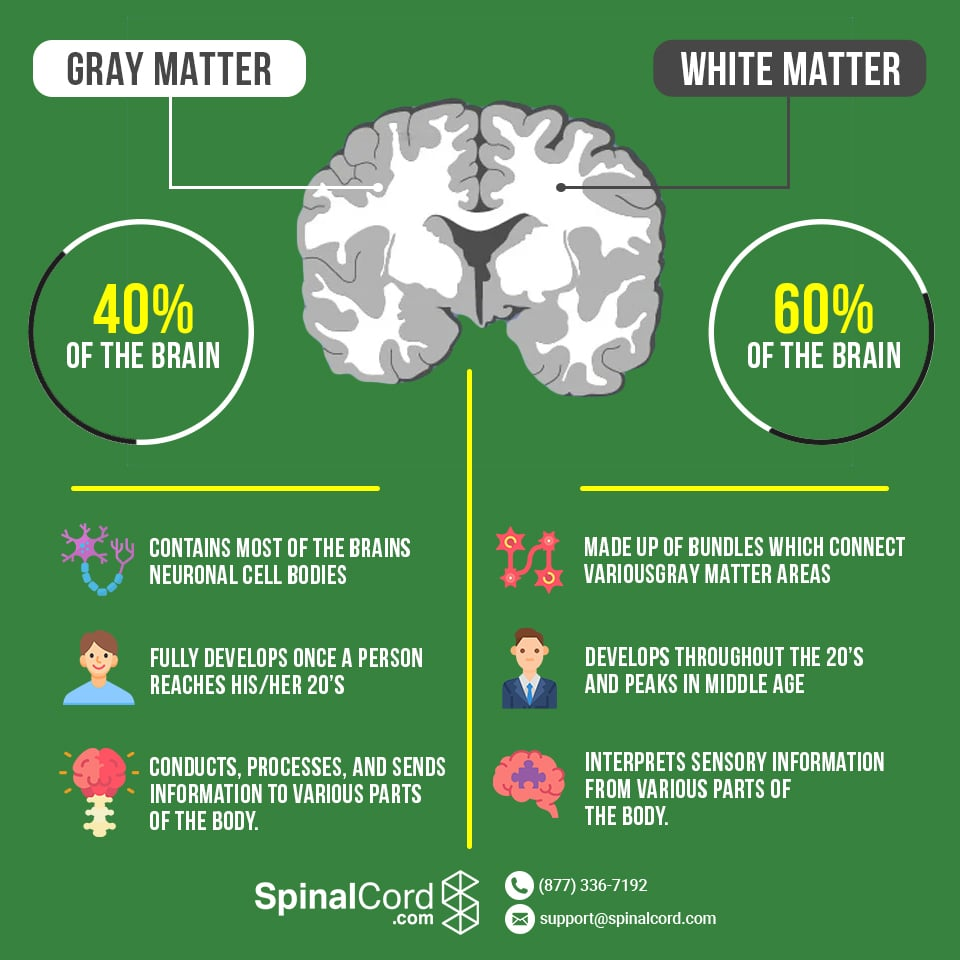
\includegraphics[width=0.5\textwidth]{assets/matter.png}
\caption{Brain matter}
\end{figure}

\begin{figure}[h]
\centering
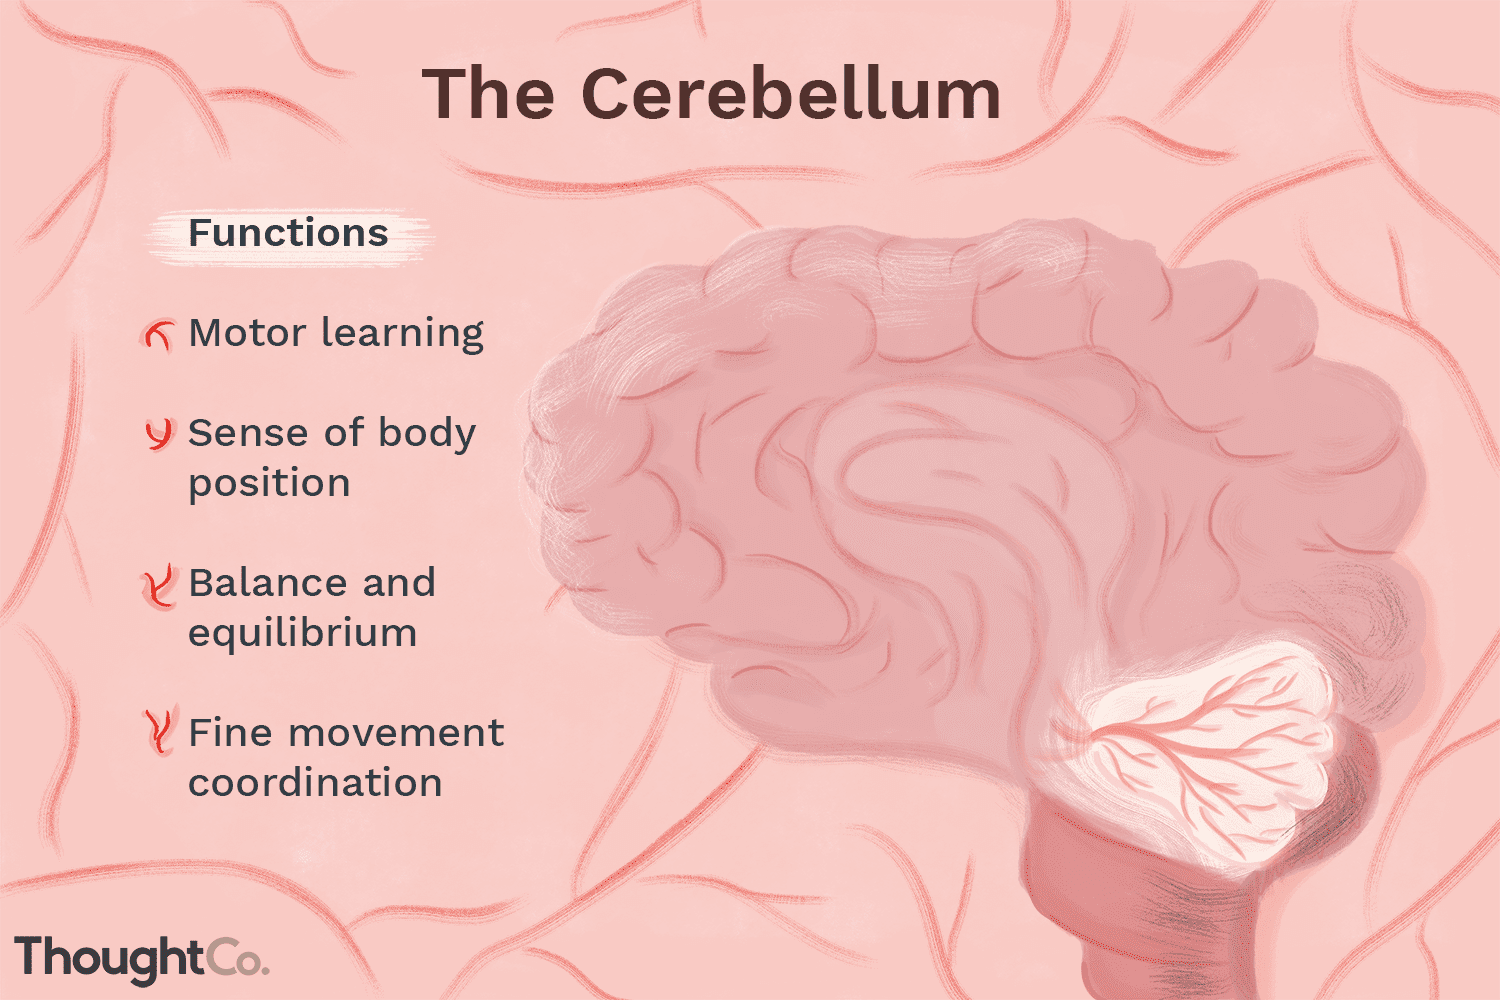
\includegraphics[width=0.5\textwidth]{assets/cerebellum.png}
\caption{Cerebellum}
\end{figure}

\begin{figure}[h]
\centering
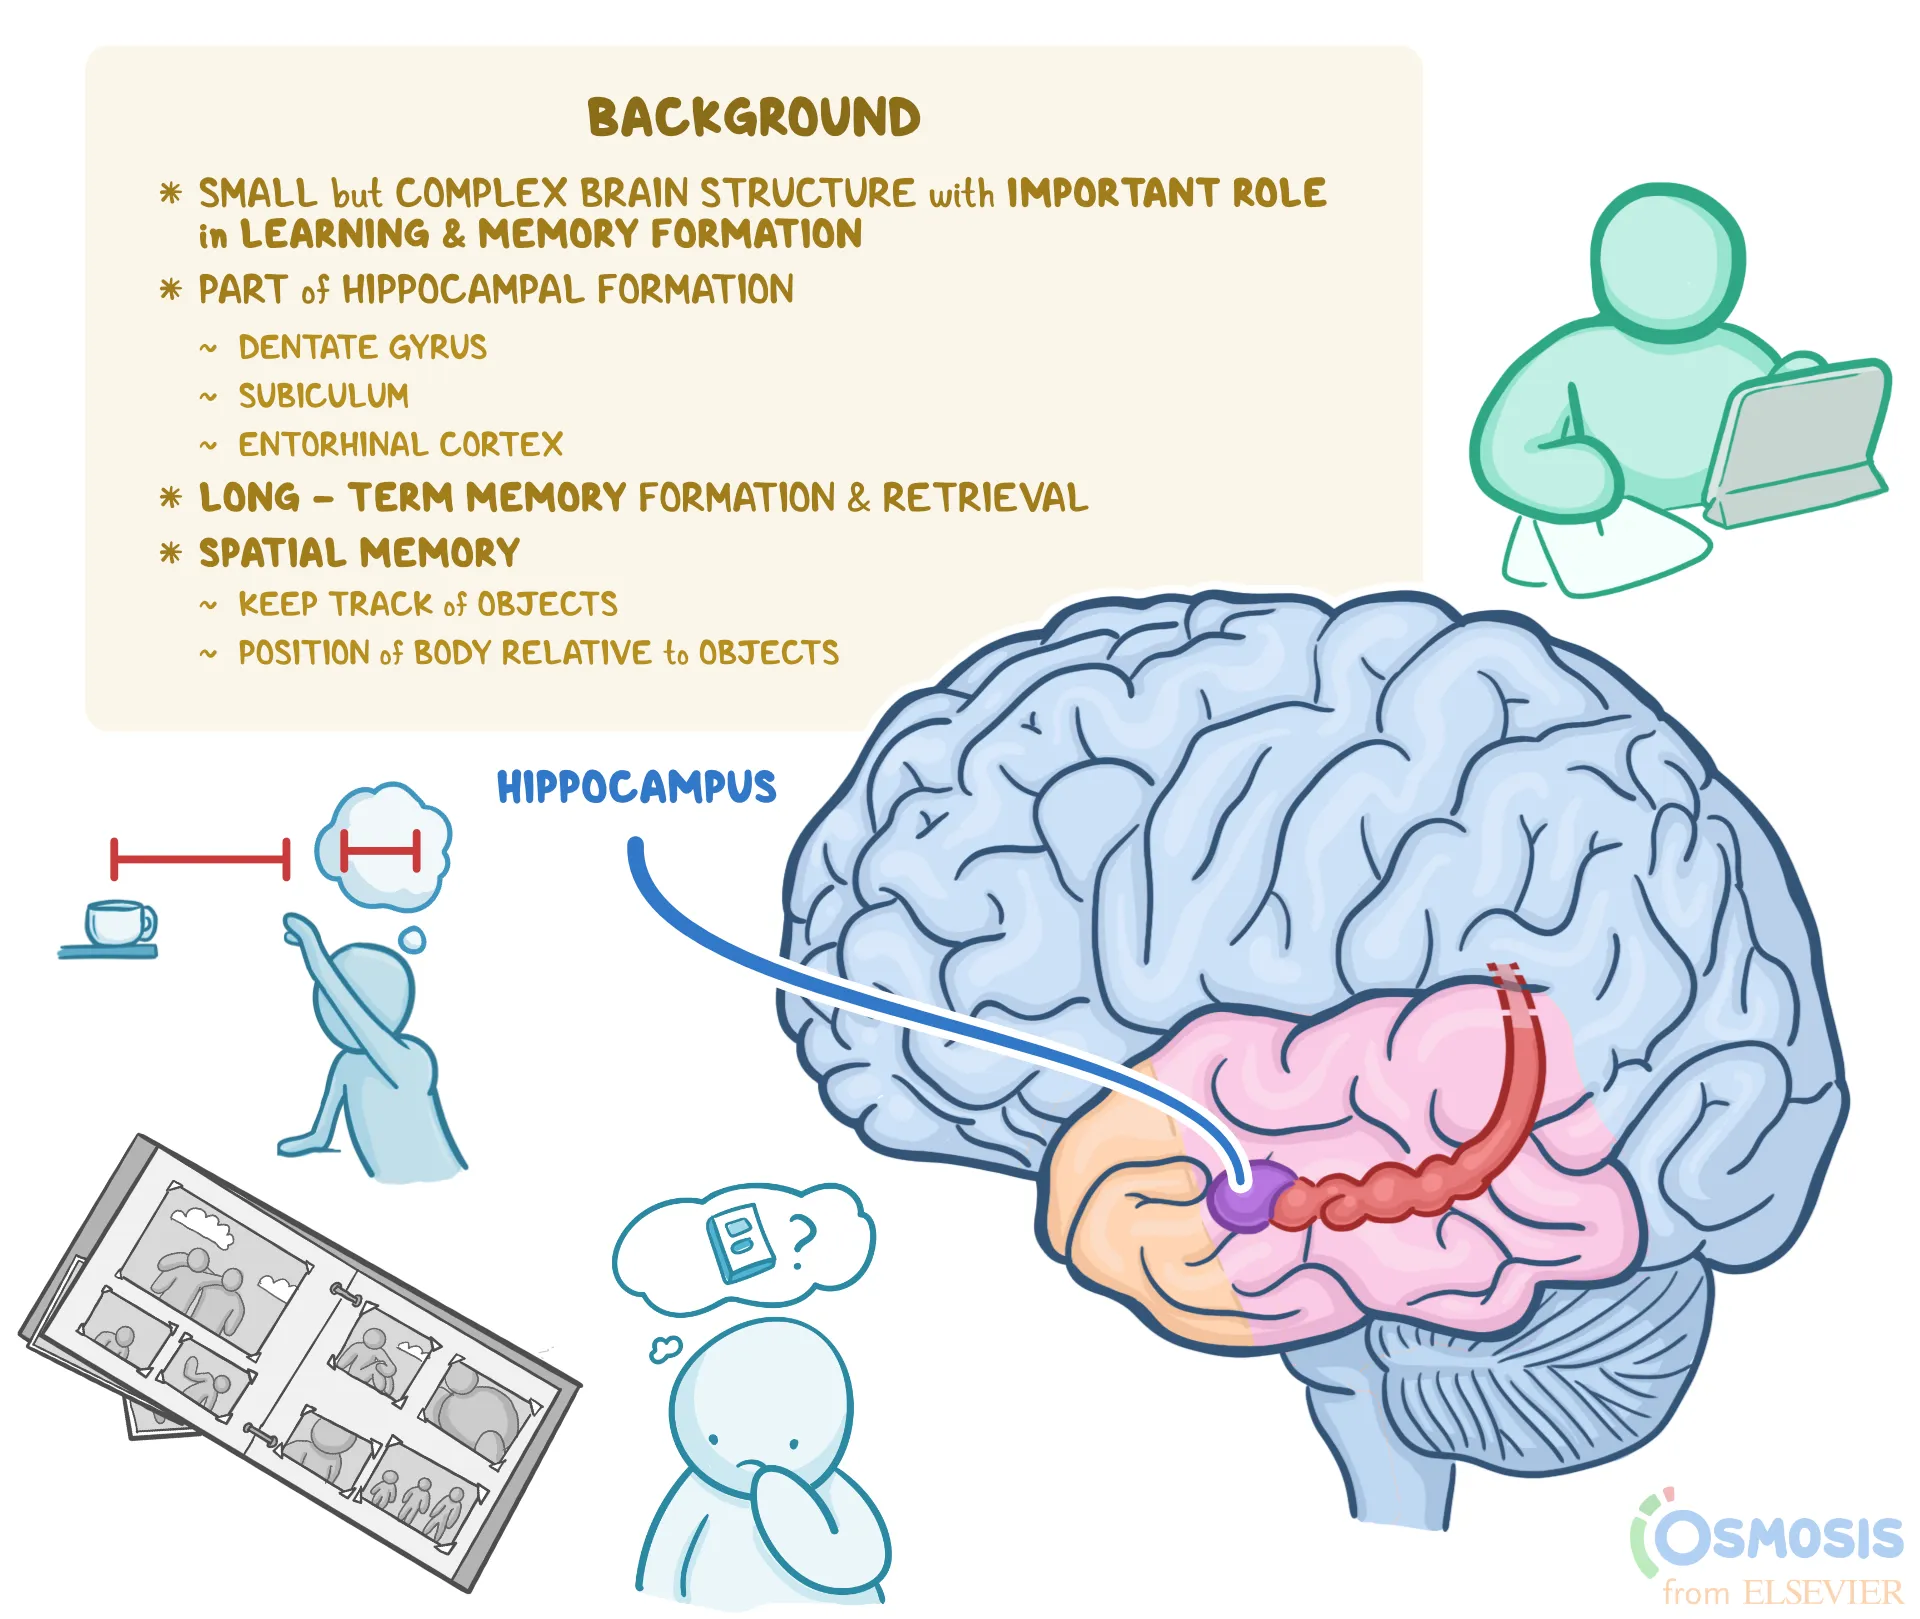
\includegraphics[width=0.5\textwidth]{assets/hippocampus.png}
\caption{Hippocampus}
\end{figure}

\begin{figure}[h]
\centering
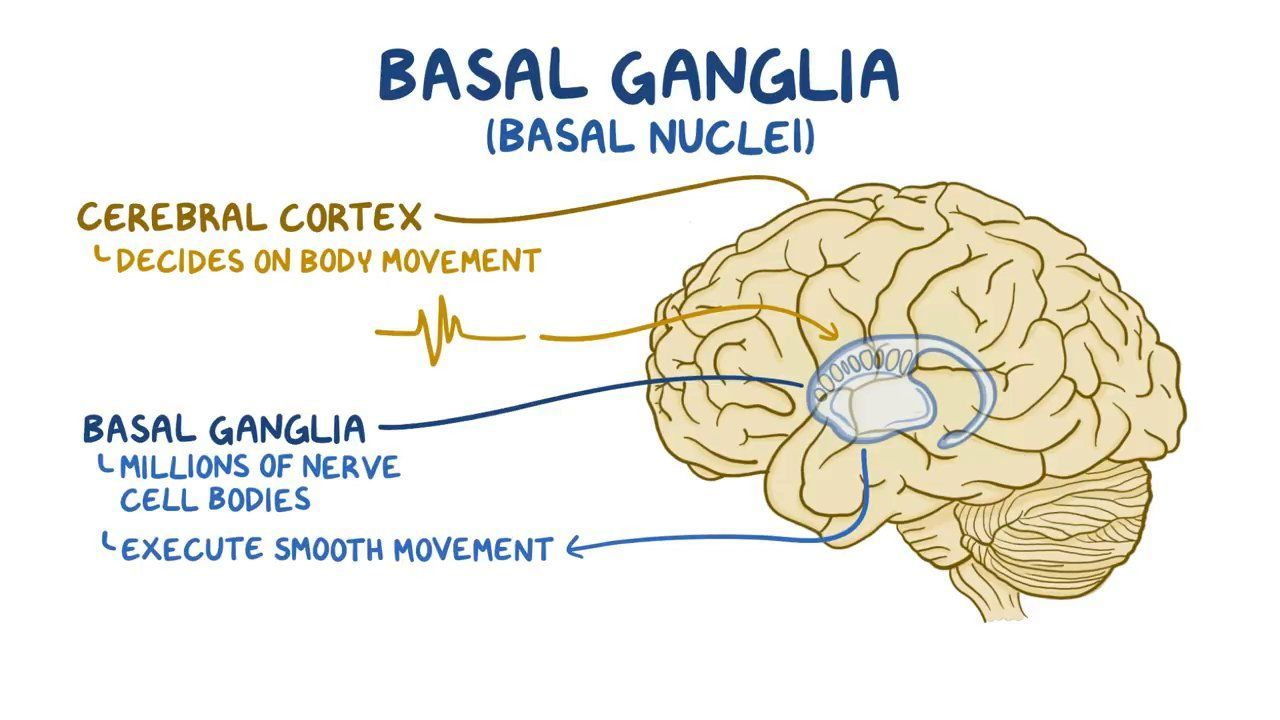
\includegraphics[width=0.5\textwidth]{assets/basalGanglia.png}
\caption{Basal Ganglia}
\end{figure}

\noindent sub-cortical structure significantly involved in motor learning and control. Degeneration of a subset of dopaminergic neurons in the basal ganglia results in Parkinson's disease.

\begin{figure}[h]
\centering
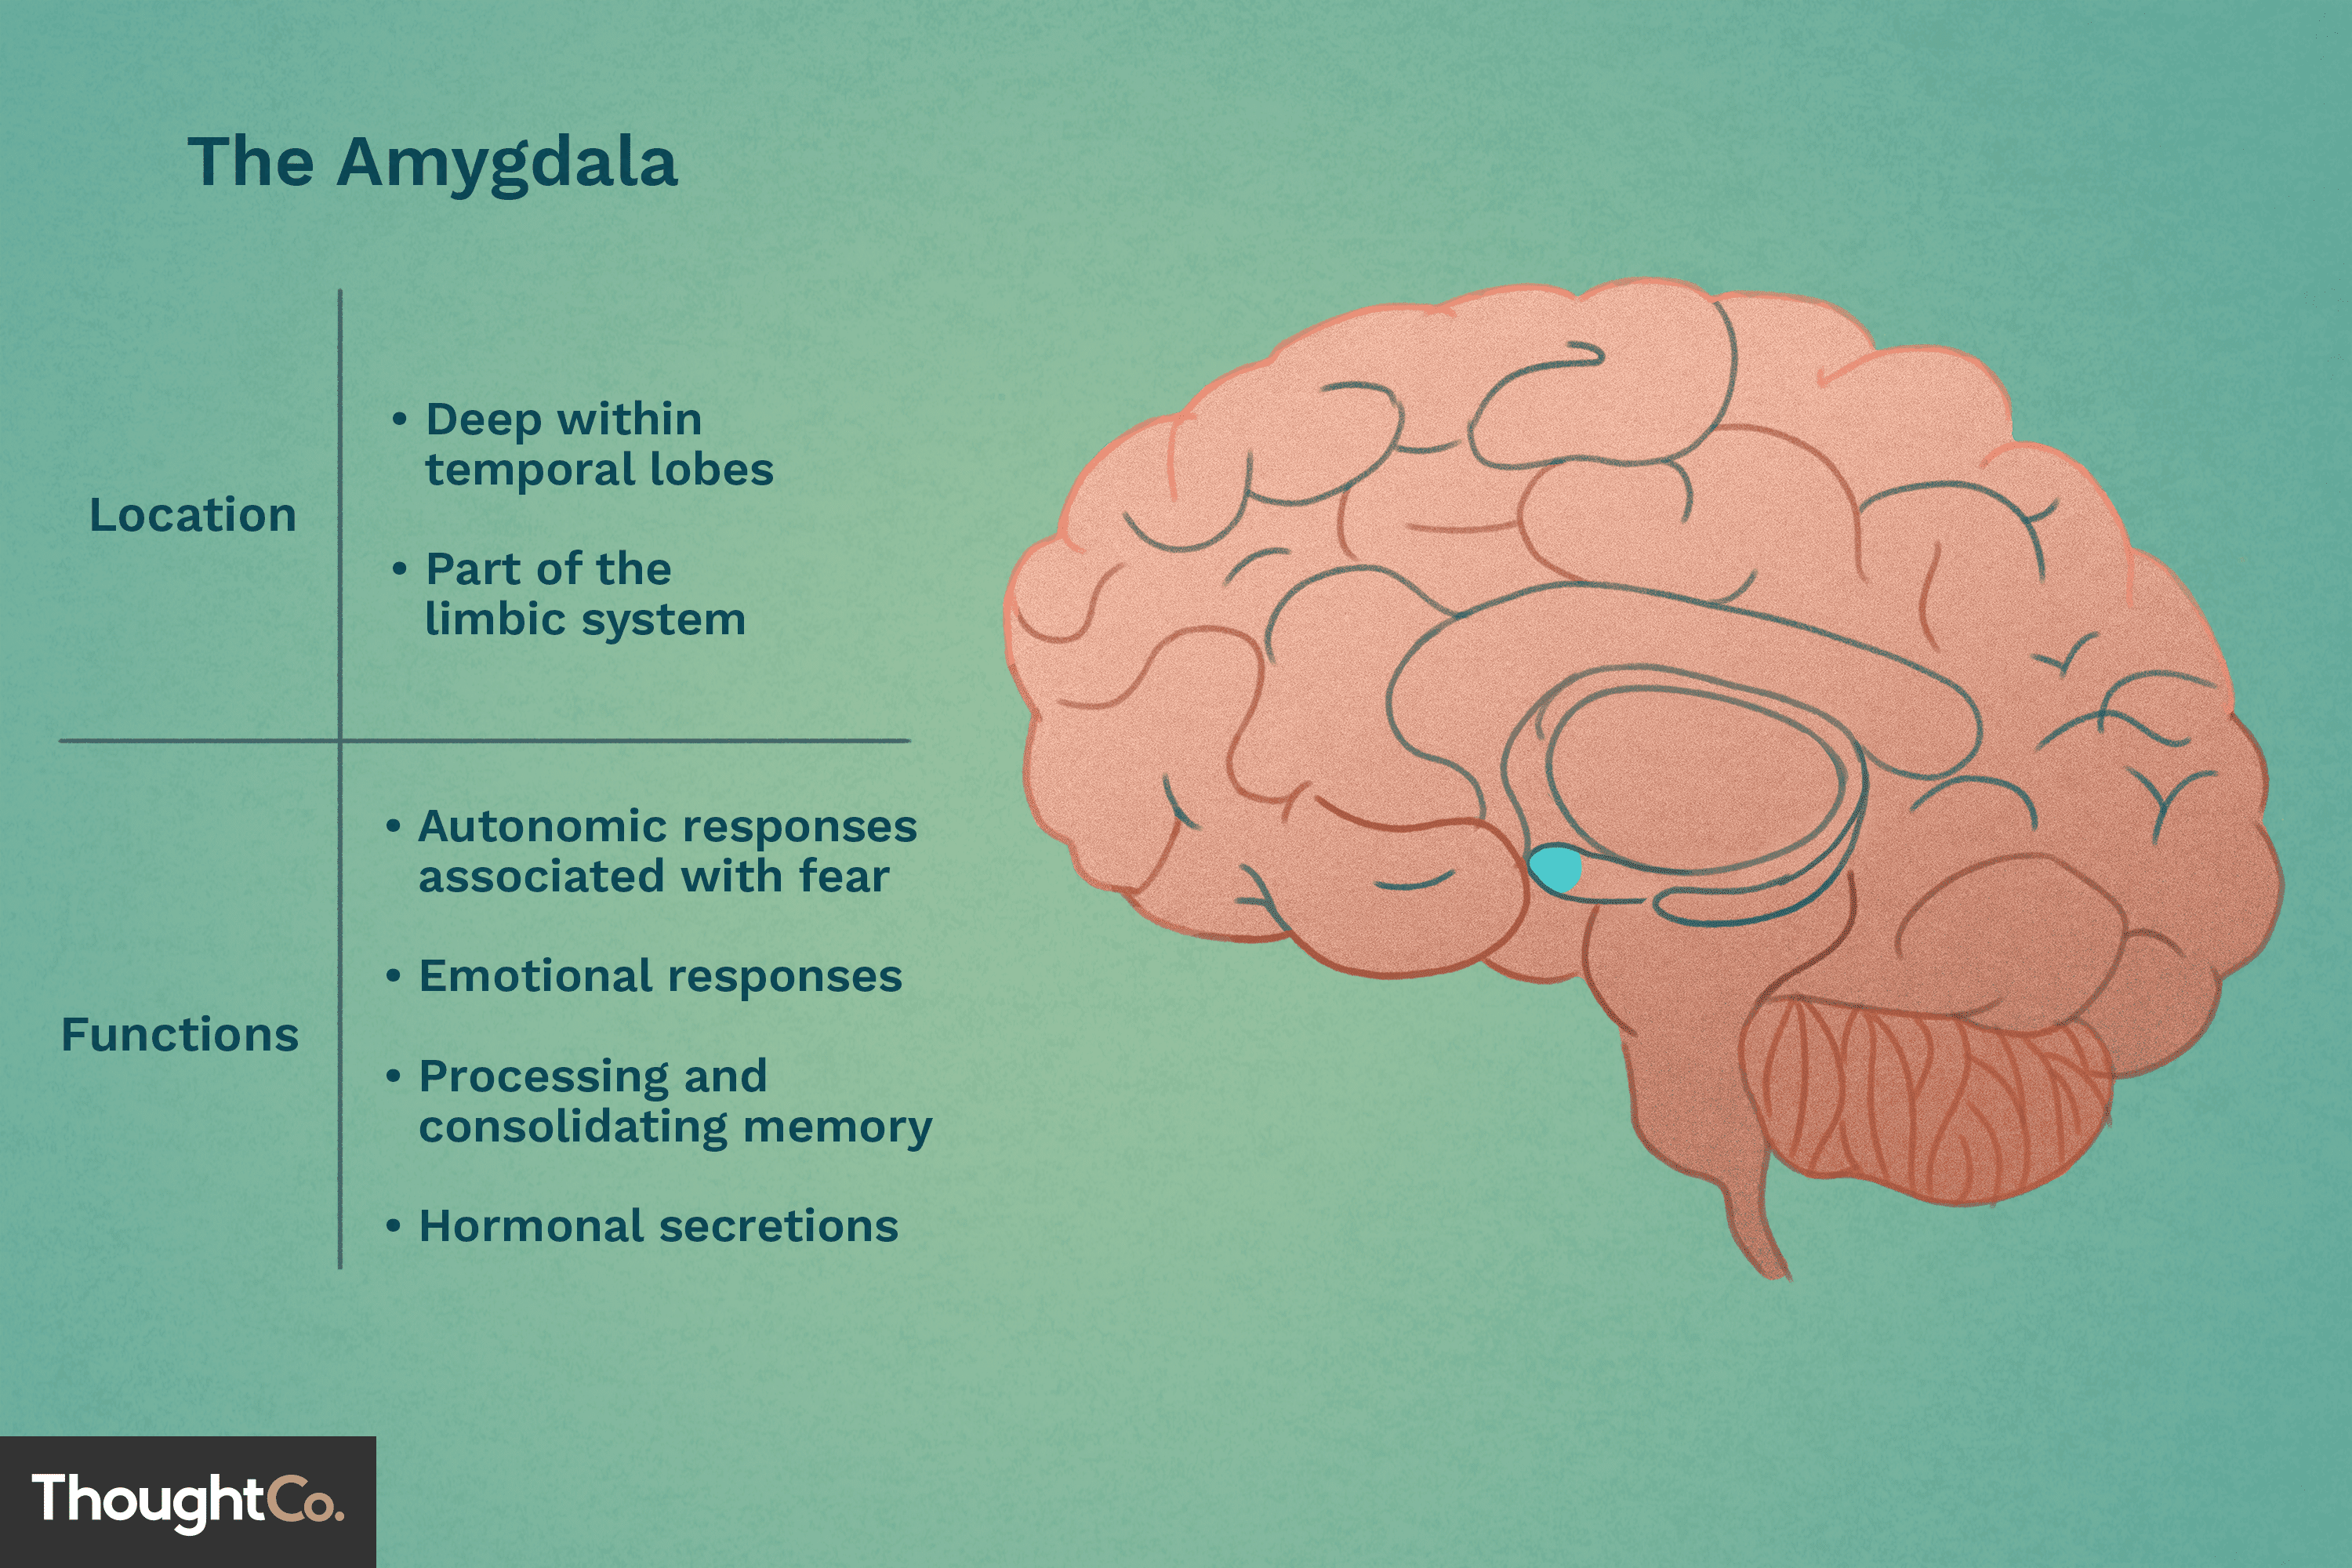
\includegraphics[width=0.5\textwidth]{assets/amygdala.png}
\caption{Amygdala}
\end{figure}

\noindent centre for emotional processing and is strongly linked to the olfactory senses (sense of smell).

\begin{figure}[h]
\centering
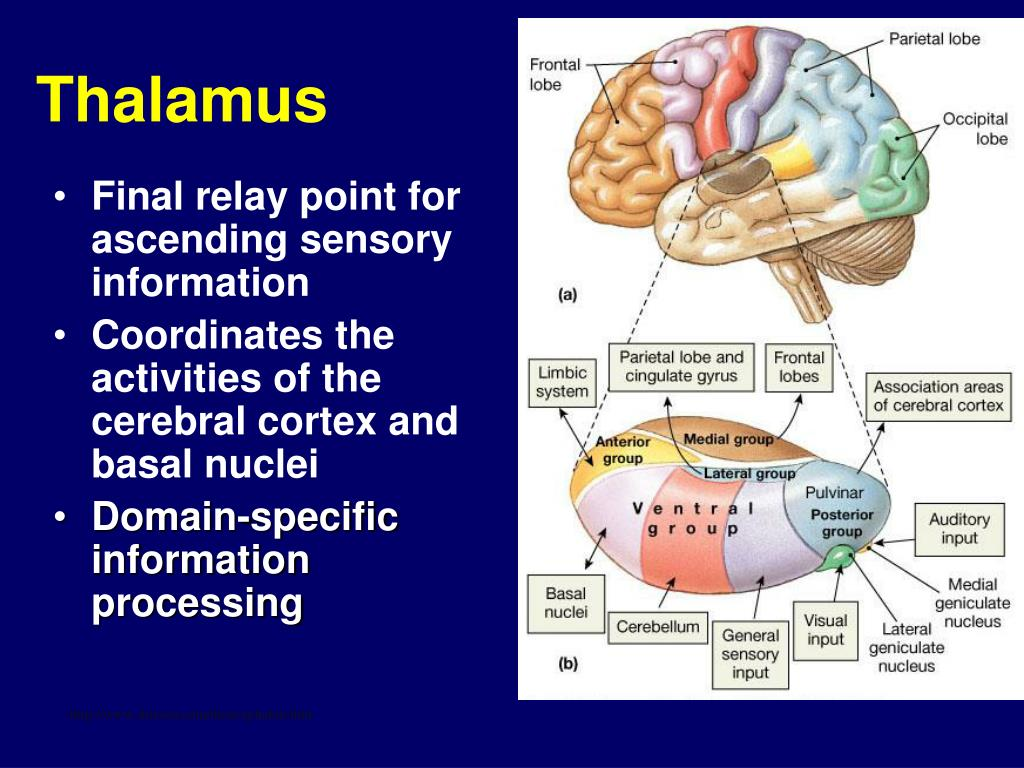
\includegraphics[width=0.5\textwidth]{assets/thalamus.png}
\caption{Thalamus}
\end{figure}

\noindent composed of several nuclei which act as relay stations to transmit information to and from neocortex.

\begin{figure}[h]
\centering
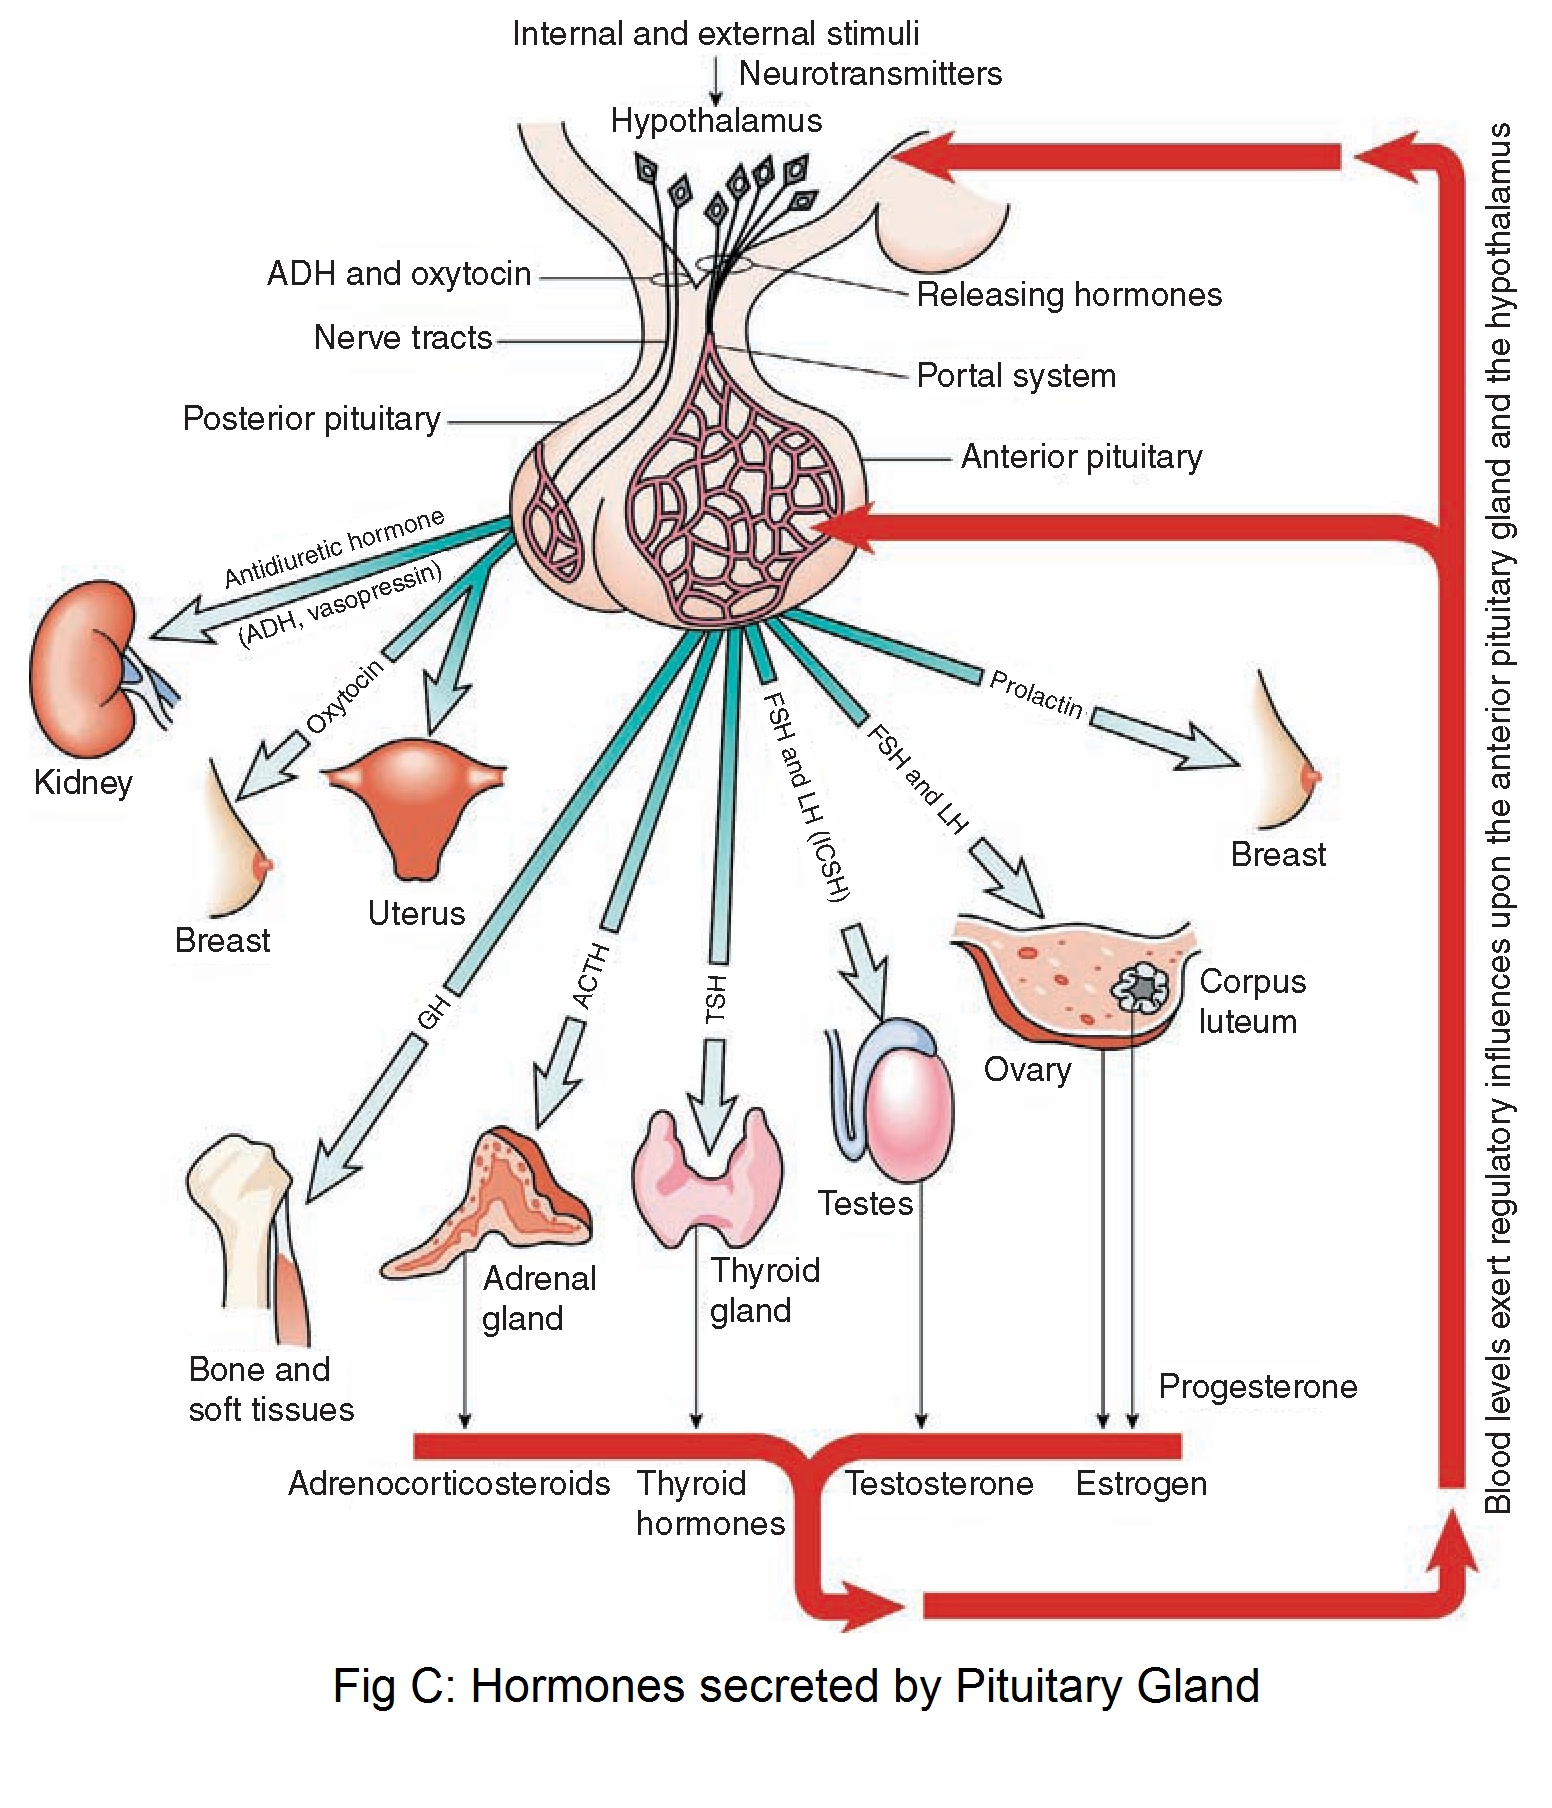
\includegraphics[width=0.5\textwidth]{assets/pituitary.png}
\caption{Pituitary gland}
\end{figure}

\begin{figure}[h]
\centering
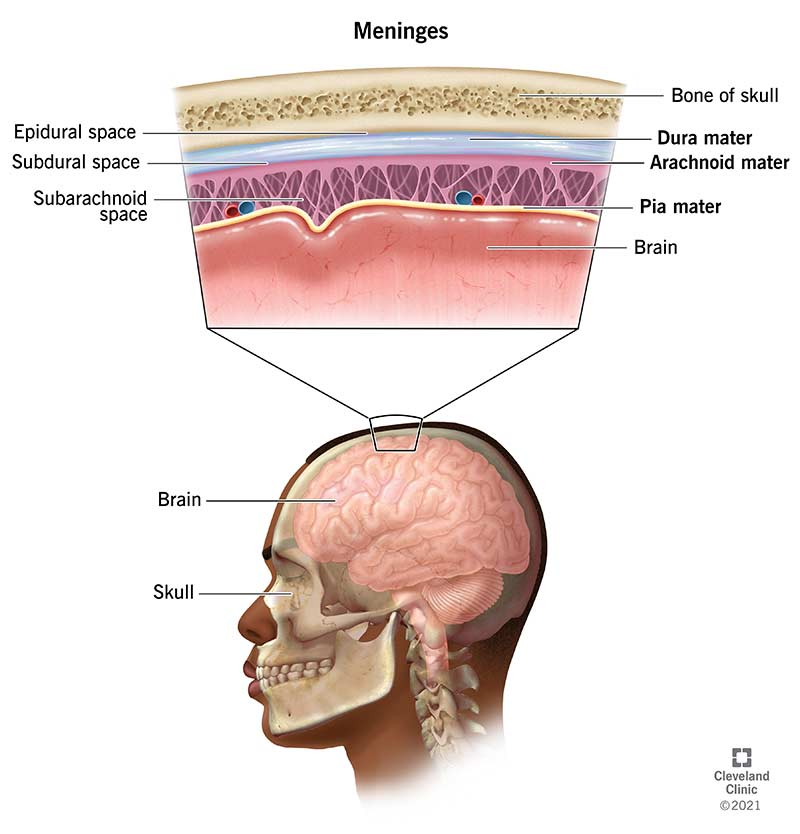
\includegraphics[width=0.5\textwidth]{assets/menings.png}
\caption{Meninges}
\end{figure}

\noindent The brain and spinal cord are protected by three layers collectively known as meninges:

\begin{itemize}
    \item dura-mater: A thick leather-like inelastic layer present directly below the bone.
    \item arachnoid-mater: A thin, delicate, middle layer present directly below the dura-mater. Has spider web like filamentous extensions into the sub-arachnoid space which reach the pia-mater
    \item pia-mater: A thin, delicate, translucent layer that directly lines the gyri/sulci of the brain, and the spinal cord. Rich in blood-vessels that supply oxygen and nutrients to the brain. Functionally, it forms the blood brain barrier (BBB).
\end{itemize}

\noindent \textbf{Diencephalon Regions}

Thalamus: composed of several nuclei which act as relay stations to transmit information to and from neocortex.

Hypothalamus: required for regulation of autonomic bodily functions

Pituitary Gland: regulation of the endocrine (hormonal) system

\begin{figure}[h]
\centering
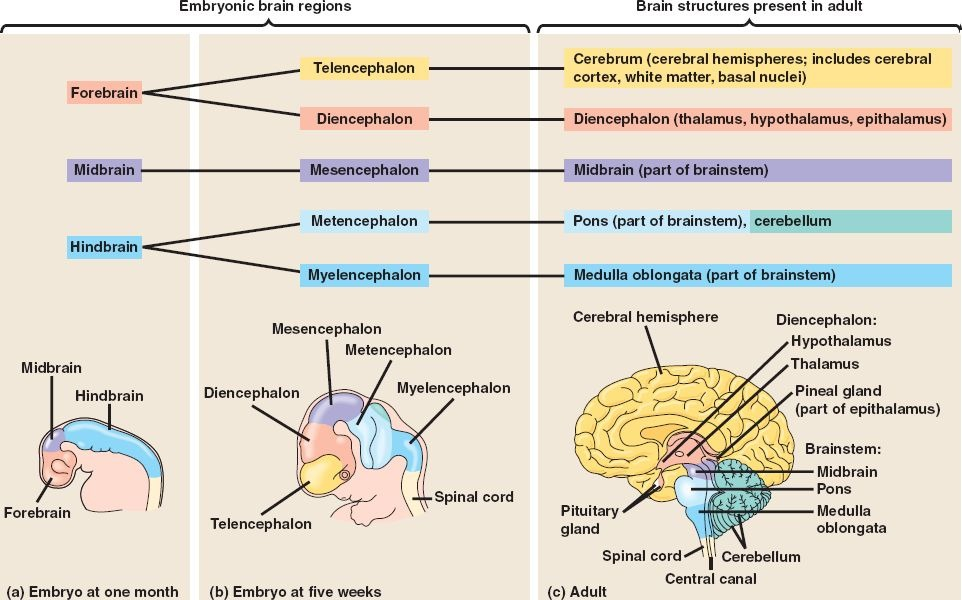
\includegraphics[width=0.5\textwidth]{assets/development.png}
\caption{Brain development}
\end{figure}

\noindent Forebrain (Prosencephalon) which can be further sub-divided into:
\begin{itemize}
    \item Telencephalon: develops into the cerebral cortex, basal ganglia, hippocampal formation, amygdala
    \item Diencephalon: gives rise to structures like the thalamus, hypothalamus and the pituitary gland.
\end{itemize}

\noindent Midbrain (Mesencephalon) tectum and tegmentum, which exist in all vertebrate brains. The tectum in the mammalian brain consists of the superior colliculus and the inferior colliculus.

\noindent Hindbrain (Rhombencephalon) consists of the Metencephalon (develops into the pons, cerebellum) and the Myelencephalon (develops into the medulla oblongata)

\begin{figure}[h]
\centering
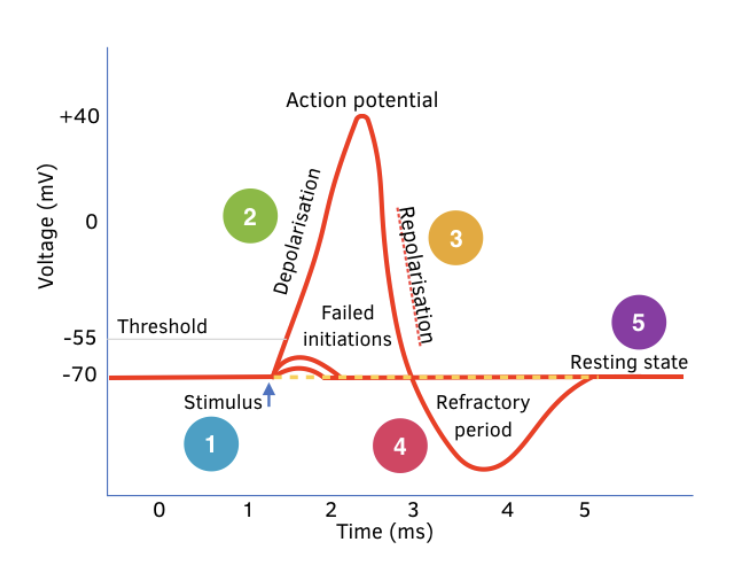
\includegraphics[width=0.5\textwidth]{assets/polarization.png}
\caption{Neuron polarization}
\end{figure}

\noindent Neurons are hyperpolarized which means they have a resting potential of -70 mV within and 0 mV outside of them. Hyperpolarization refers to an increase in membrane potential whereas depolarization refers to a decrease in membrane potential

\noindent Action potentials are all or nothing operations which have four components which take place over the course of 1-2 ms:
Depolarization: Depolarization is when a change occurs inside a cell that causes the distribution of electric charges to alter, leaving the cell with a less negative charge than the outside. Numerous cell functions, cell-cell communication, and the general physiology of an organism all depend on depolarization

\section*{Exam Questions}

\begin{enumerate}
    \item \textbf{Grid Cells}: Grid cells are types of neurons found in the brains of many animals, including humans, that allow for spatial navigation and are thought to form part of the brain's positioning system. These cells are located in the entorhinal cortex and exhibit a unique pattern of activity that corresponds to multiple, evenly spaced locations in an environment, forming a grid-like structure. This pattern helps in self-positioning and navigation by providing a metric for spatial coding. Understanding grid cells involves knowing how their firing patterns contribute to the neural code for representing space in the brain.

    \item \textbf{Brain Size Scaling with Species Size}: The relationship between brain size and the size of a species, also known as allometric scaling, is an important area of study in comparative neuroscience. Generally, brain size increases with body size, but not in a simple linear way; instead, it follows a power law where the exponent is less than one, indicating that larger animals have larger brains but not proportionally to their body size. This is sometimes expressed as the encephalization quotient (EQ), which measures brain mass relative to an expected value for a given body mass.

    \item \textbf{Perceptrons and XOR Function}: A perceptron is a simple linear classifier that can only solve linearly separable problems. The XOR function is not linearly separable, which means a single perceptron cannot compute an XOR function. However, a multi-layer network with at least one hidden layer (also known as a multi-layer perceptron) can solve the XOR problem by creating a non-linear decision boundary.

    \item \textbf{Convergence in Hopfield Networks}: A given state in a Hopfield network will converge to a stable state if it's close to one of the stored patterns (memories) or local minima of the energy function. To determine which of the four states will converge to a stable state, you would analyze the energy function of the Hopfield network and determine which states are local minima.

    \item \textbf{Output from an Integrate-and-Fire Circuit}: An integrate-and-fire neuron model is a simplified representation of a neuron that accumulates input signals until it reaches a threshold, at which point it 'fires' (generates an action potential) and then resets. The output of such a circuit is typically a series of spikes or action potentials over time.

    \item \textbf{Short-Term Plasticity vs Long-Term Potentiation}: Short-term plasticity refers to transient changes in synaptic strength that occur over a short period, such as facilitation or depression due to recent activity. Long-term potentiation (LTP), on the other hand, is a long-lasting increase in synaptic strength following high-frequency stimulation, which is a mechanism underlying learning and memory.

    \item \textbf{Tuning Curves (Population Codes)}: A tuning curve represents the response of a neuron to a range of stimuli, showing how the firing rate of the neuron changes with different stimulus values. It's an essential concept in understanding population coding, where the combined activity of multiple neurons with different tuning properties can encode complex information, such as sensory inputs.

    \item \textbf{Activation Levels from a 2D Stimuli Input}: The question likely refers to interpreting a heatmap or graph showing how a neuron's activation level varies with two-dimensional stimulus input. Areas of highest activation would correspond to the preferred stimulus of the neuron, while areas of lowest activation would correspond to non-preferred stimuli.

    \item \textbf{Action Potential Annihilation Due to Refractory Period}: The refractory period is the time immediately following an action potential during which a neuron is unable to fire another action potential. This refractory period prevents the backward propagation of the action potential and ensures unidirectional travel along an axon.

    \item \textbf{Cable Equation and EPSP Potential}: The cable equation describes how electrical signals decay as they travel through the dendrites and axons of neurons. An excitatory postsynaptic potential (EPSP) is a temporary increase in postsynaptic membrane potential due to the flow of positively charged ions into the cell. The potential is highest at the site of the synapse and decreases with distance from the point of synaptic contact due to the cable properties of the neuron.
\end{enumerate}

- \textbf{Graph of LTP Changes}: Long-term potentiation (LTP) is typically visualized by plotting the post-synaptic response strength over time. A normal graph of LTP would show a stable baseline of synaptic response followed by a sudden and sustained increase in response following a high-frequency stimulus. A modified graph might show a diminished LTP response, possibly due to pharmacological intervention, genetic modification, or pathology. Analyzing such graphs would involve noting differences in the magnitude, onset, and duration of LTP.

- \textbf{Injecting Two Currents at Both Ends}: When injecting two currents into the ends of a neuron, the interaction of the currents will depend on the neuron's properties, such as membrane resistance and capacitance. The currents will spread passively inside the neuron and decay over distance. The actual effect also depends on whether the currents are excitatory or inhibitory and their relative strengths and timings.

- \textbf{Reversal Potential of a Single Ion}: The reversal potential (also known as equilibrium potential) for a single ion can be calculated using the Nernst equation:
\[
E_{\text{ion}} = \frac{RT}{zF} \ln\left(\frac{[\text{ion}]_{\text{outside}}}{[\text{ion}]_{\text{inside}}}\right)
\]
where $R$ is the gas constant, $T$ is the temperature in Kelvin,$z$ is the valence of the ion, $F$ is the Faraday constant, and $[\text{ion}]_{\text{outside}}$ and $[\text{ion}]_{\text{inside}}$ are the external and internal concentrations of the ion, respectively.

- \textbf{Property About Brains}: Humans do not have the largest brains in absolute size—that distinction goes to larger animals like whales or elephants. However, humans do have a high encephalization quotient (EQ), which is a measure of brain size relative to what would be expected for an animal of our body size. Humans also do not have the most neurons; for instance, some species of whales have more neurons due to their larger brains. Brain size generally scales with body size, but not in a simple linear relationship.

- \textbf{Resting Potential and Reversal Potential}: The resting potential of a cell is closest to the reversal potential of the ion that has the highest permeability across the cell membrane, which is typically potassium (K+). This is due to the fact that the resting membrane is most permeable to K+, and the movement of K+ ions out of the cell has the most significant effect on the resting potential.

- \textbf{Ion Flow During Resting/Polarization/Depolarization}: During the resting state, K+ ions flow out of the cell, and Na+ ions flow into the cell, but the K+ flow is dominant, keeping the membrane potential close to the K+ reversal potential. During depolarization, Na+ ions flow rapidly into the cell, making the inside more positive. During repolarization, K+ ions flow out of the cell, restoring the negative internal environment.

- \textbf{Electrical Synapses vs. Chemical Synapses}: Electrical synapses are direct connections between cells that allow for the rapid transfer of electrical signals via gap junctions. They are bidirectional and can synchronize the activity of connected neurons. Chemical synapses, on the other hand, use neurotransmitters to transfer signals from one neuron to another, are unidirectional, and have a synaptic delay. They are also modifiable, meaning they can be strengthened or weakened over time, which is the basis for learning and memory.

- \textbf{Loewi's Experiment}: Otto Loewi demonstrated chemical neurotransmission by showing that stimulating one frog's heart could release a substance (later identified as acetylcholine) that, when transferred to another frog's heart, slowed its rate. This experiment provided evidence that nerve impulses could affect heart rate through chemical means.

- \textbf{Properties of the PLA (Perceptron Learning Algorithm)}: The PLA is an algorithm used to train perceptrons. It iteratively adjusts the weights and bias of the perceptron based on its output errors, moving the decision boundary towards the optimal position that separates the classes in linearly separable data sets.

- \textbf{Hopfield Networks}: Hopfield networks have discrete-time dynamics with binary threshold units, are fully connected, and have symmetric weight matrices. They serve as associative memories by converging to stable states, which represent the memorized patterns.

- \textbf{Perceptrons vs. Logic Gates}: Perceptrons are a simple model of a neuron that can learn to make decisions by adjusting its weights in response to training data. Logic gates, however, are fixed-function devices that perform basic logical operations like AND, OR, and NOT without the ability to learn. Perceptrons can implement certain logic gates (like AND and OR for linearly separable patterns) but not others

\subsection*{Since this is a linear system, which of the following will always be true?}

\begin{enumerate}
    \item The weighting coefficients always lie on a straight line
      \begin{itemize}
        \item False
      \end{itemize}
    \item If you scale the input by a constant, the output will be scaled by the same constant
      \begin{itemize}
        \item True
      \end{itemize}
    \item The output of a sum of different inputs is equal to the sum of the outputs of each of the individual inputs
      \begin{itemize}
        \item True
      \end{itemize}
    \item The filter is a linear function of the input
      \begin{itemize}
        \item False
      \end{itemize}
\end{enumerate}

\subsection*{Which of the following inputs might cause a linear system with a positive filter to predict a negative rate?}

\begin{enumerate}
    \item An input that slowly varies between a large positive value and a large negative value
      \begin{itemize}
        \item true
      \end{itemize}
    \item A positive input that decays to zero over time
    \item A positive input with a discontinuity
    \item None of these
\end{enumerate}

\begin{figure}[h]
\centering
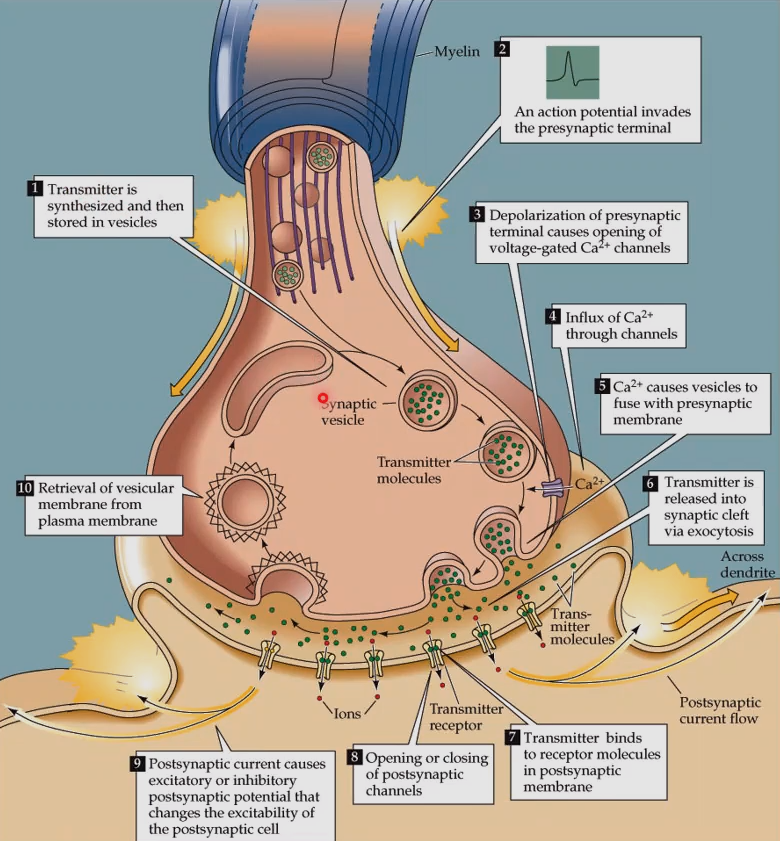
\includegraphics[width=0.5\textwidth]{assets/chemical-synapses.png}
\caption{Chemical synapses}
\end{figure}

\subsection*{Chemical transmission}

\begin{itemize}
    \item Contrary to electrical transmission multiple steps are required to release transmitter chemicals and for them to act on postsynaptic receptors, resulting in a time delay
    \item Directional, select localization of release machinery to presynaptic terminals and receptors to postsynaptic specializations
    \item can change sign by release of inhibitory transmitter
    \item highly modulatable as it has many steps presynaptic terminal and at the postsynaptic sites
\end{itemize}

\begin{figure}[h]
\centering
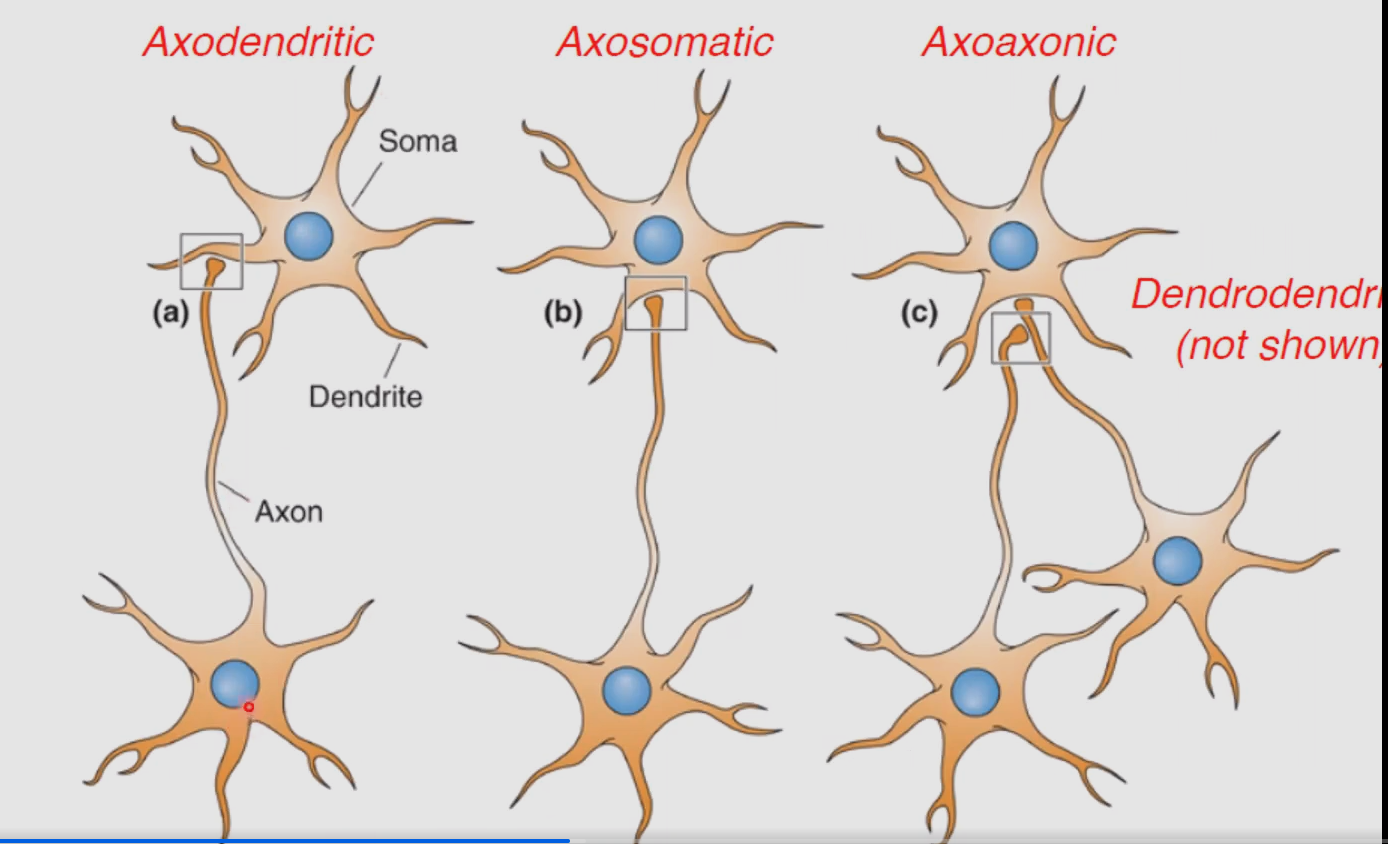
\includegraphics[width=0.5\textwidth]{assets/types-of-synapses.png}
\caption{Types of synapses}
\end{figure}

\subsection*{Steps to chemical synaptic transmission}

\begin{itemize}
    \item First need to bring the presynaptic neuron to threshold at axon hillock
    \item Conduction down axon length $R * C$ dependent
    \item Opening of voltage gated Ca channels
    \item Diffusion and action of Ca at release machinery
    \item Exocytosis and diffusion of transmitter in cleft
    \item Activation of postsynaptic receptors
\end{itemize}

\subsection*{Criteria that define a neurotransmitter}

\begin{enumerate}
    \item must be present at presynaptic terminal
    \item must be released by depolarization, $Ca^{++}$-dependent
    \item specific receptors must be present
\end{enumerate}

\begin{figure}[h]
\centering
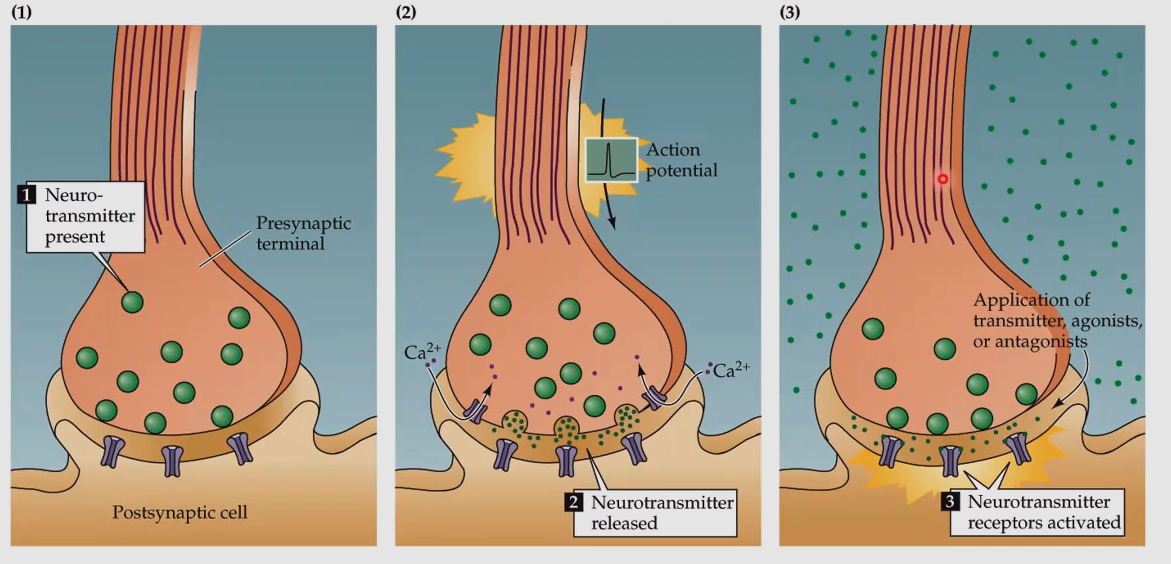
\includegraphics[width=0.5\textwidth]{assets/neurotransmitter.png}
\caption{Neurotransmitter}
\end{figure}

\subsection*{Standard Katz (Quantal) Model of Synaptic Transmission}

\begin{itemize}
    \item One packet of neurotransmitter = 1 quantum
    \item AP transiently increases in the probability of releasing NX quanta
    \item Several quanta are available to be released
    \item Each quantum gives approximately the same postsynaptic response called the Quantal Amplitude
    \item The average number of quanta released, $m = np$
      \begin{itemize}
        \item where $n$ = number of quanta available for release
        \item $p$ = their average release probability
      \end{itemize}
\end{itemize}

\subsection*{CNS synapses and quanta}

\begin{itemize}
    \item at CNS synapses with only a single release site, changing the probability of release (i.e. changing calcium concentration) does not effect the amplitude of the response (as only zero or one vesicle is released in theory)
    \item at CNS synapses with multiple release sites, changing release probability can change the postsynaptic response amplitude as more transmitter is released (graded quantal levels)
    \item at the NMJ a single nerve can elicit a postsynaptic AP given multiquantal release, while at the CNS synapse (with low number of release sites) multiple synapses must cooperate, forces a network
\end{itemize}

\subsection*{Docked Synaptic Vesicles}

Define the number of readily releasable vesicles a synapse has available. A consequence of having of limited number is depletion at high stimulus frequency, CNS synapses may have only a small number of docked vesicles on the order of 5-10 vesicles for a hippocampal CA1 synapse

\begin{figure}[h]
\centering
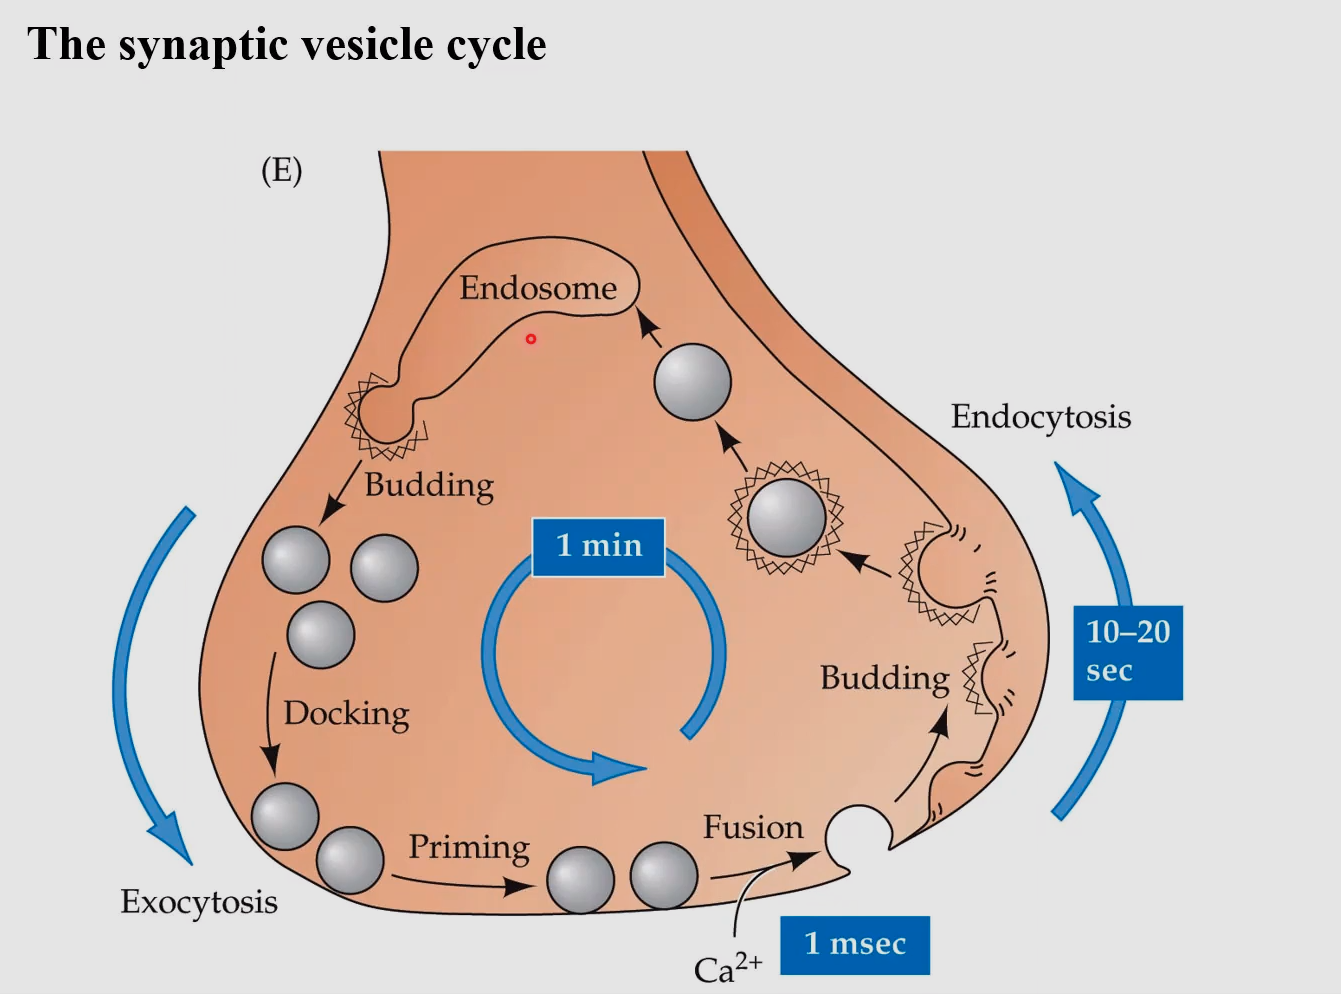
\includegraphics[width=0.5\textwidth]{assets/synaptic-vesicle-cycle.png}
\caption{Synaptic vesicle cycle}
\end{figure}

\end{document}
